\documentclass[a4paper, 12pt]{report}

\usepackage{hyperref}
\usepackage{verbatim}
\usepackage{titlesec}
\usepackage{graphicx}
\usepackage{caption}
\usepackage{subcaption}

\begin{document}

\section*{Simple Polygonize}

Demonstration of algorithm for finding a simple polygon that passes through given points. Implemented for CSN-523 (Computational Geometry) course assignment.

\subsection*{Algorithm}

\begin{enumerate}
\item Choose a suitable reference point (in the code, used arithmetic mean of each axis)
\item Calculate angle of line segment joining each given point to the reference point, with respect to the X axis
\item Sort the points based upon the angle of incidence calculated above
\item Join adjacent points in the sorted order using line segments
\item Join first and last point with a line segment
\end{enumerate}

\subsection*{Code}

\verbatiminput{../simple-polygonize.py}


\subsection*{License}

All parts of the code are covered under the \href{https://jay.mit-license.org/2017}{MIT License}

\subsection*{How to Run}

Simply run the \verb|simply-polygonize.py| file using \verb|python simply-polygonize.py| or \verb|python simply-polygonize.py {N}|, where \verb|N| is the number of points required.

When the program runs, it will prompt with the help text:

\begin{verbatim}
        +/- Change N
         r  randomize points
         q  quit
\end{verbatim}

Press any of the above keys to do the corresponding action.

\subsection*{Demonstration}

A video of the code in action, is available at \\ \href{https://www.youtube.com/watch?v=WXUb6b_7CIk}{https://www.youtube.com/watch?v=WXUb6b\_7CIk}

Some screenshots are shown below:


\begin{figure*}[h]
    \centering
    \begin{subfigure}[t]{0.4\textwidth}
        \centering
        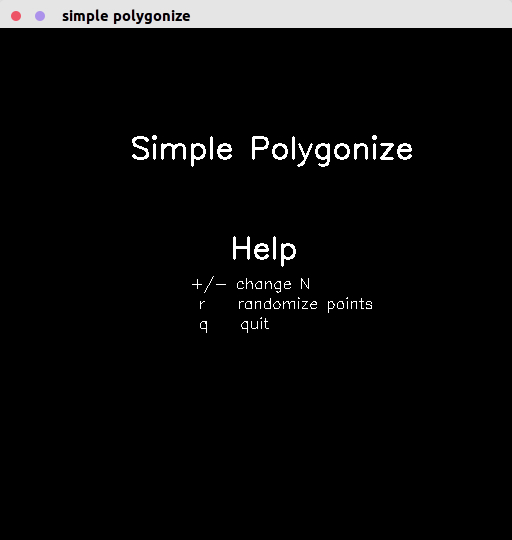
\includegraphics[width=\textwidth]{0-intro}
        \caption{Intro Screen}
    \end{subfigure}%
    ~
    \begin{subfigure}[t]{0.4\textwidth}
        \centering
        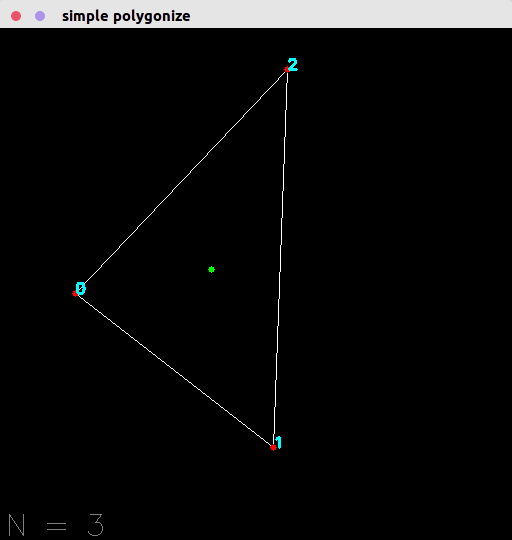
\includegraphics[width=\textwidth]{1-n3}
        \caption{N=3}
    \end{subfigure}%
    \\
    \begin{subfigure}[t]{0.4\textwidth}
    	\centering
    	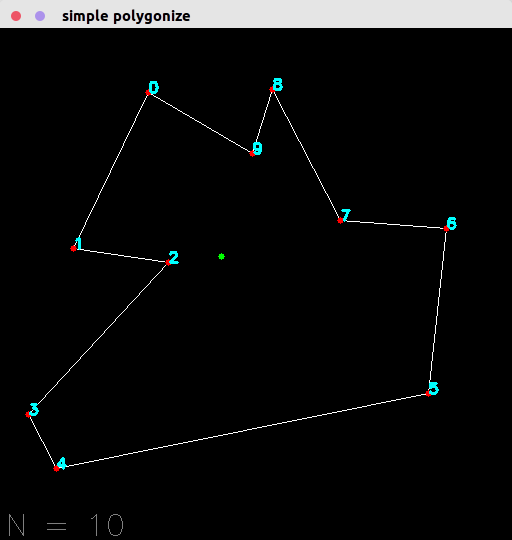
\includegraphics[width=\textwidth]{2-n10}
    	\caption{N=10}
    \end{subfigure}%
    ~
    \begin{subfigure}[t]{0.4\textwidth}
    	\centering
    	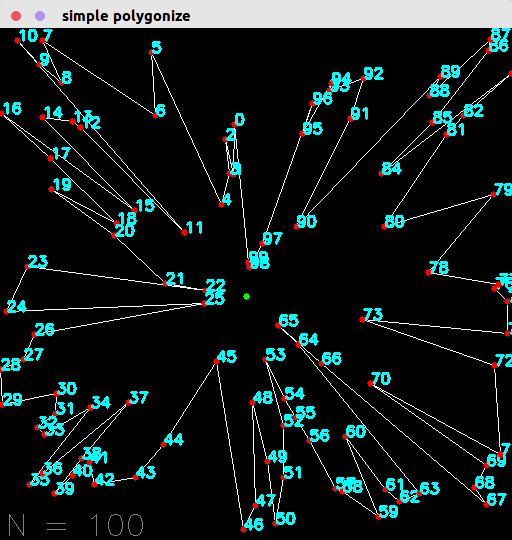
\includegraphics[width=\textwidth]{3-n100}
    	\caption{N=100}
    \end{subfigure}
\end{figure*}

\end{document}          
